\documentclass[a4paper,10pt]{article}
\usepackage[a4paper]{geometry}
\geometry{hmargin=2cm, vmargin=3cm}
\usepackage{hyperref}
\usepackage{fontspec}
\usepackage{xunicode}
\usepackage{fontspec}
\usepackage{xltxtra}
\setmainfont{Linux Libertine}
\setsansfont{DejaVu Sans}
\usepackage{polyglossia}
\setdefaultlanguage{french}
\usepackage{minted}
\usepackage{algorithm}
\usepackage{algorithmic}
\usepackage{titlesec}
\usepackage{amsmath}
\usepackage{subcaption}
\titleformat*{\section}{\large\bfseries\sffamily}
\titleformat*{\subsection}{\bfseries\sffamily}

\begin{document}
% Page de présentation
\begin{center}
\thispagestyle{empty}
~\\
\vspace{5cm}
{\Huge \sffamily Rapport de théorie des graphes}\\
\vspace{5cm}
Élie \textsc{Bouttier} \& Franklin \textsc{Delehelle}\\
\end{center}
\newpage

% Début effectif du document
\section{Introduction}
Nous avons décidé d'utiliser l'opportunité qui nous était offerte de travailler sur ce projet pour implémenter 
un algorithme de \emph{pathfinding} pour un robot qui participera à la coupe de France de robotique 2013.

\section{L'algorithme}
Nous avons choisi d'utiliser JPS, un algorithme très récent, puisque publié en

2011\footnote{http://grastien.net/ban/articles/hg-aaai11.pdf}, qui permet d'optimiser l'algorithme bien connu d'A* en ne le 
développant que là où nécessaire ; pour cela, il utilise deux règles :
\begin{description}
\item[règle d'élagage] pour tout point $x$ atteint depuis $p$, on supprime tout ses voisins $n$ dont soit le chemin $(p,y,n)$
ou $(p,n)$ est plus court que $(p,x,n)$, ou bien dont les chemins $(p,y,n)$ et $(p,x,n)$ ont la même longueur, mais dont le
chemin $(p,y,n)$ comporte un mouvement diagonal plus tôt que $(p,x,n)$. Les voisins conservé après cet élagage sont appelés 
\emph{voisins naturels} de $x$. Les voisin supplémentaires entre les cas où $x$ est entouré de vide et le voisinage de $x$ 
contient un obstacle sont appelés \emph{voisins forcés}.

\item[règle de saut] les sauts consistent, à direction donnée, à explorer les voisins non élagués du nœud
de départ
\begin{figure}[h]
\centering
\begin{subfigure}{.3\textwidth}
\centering
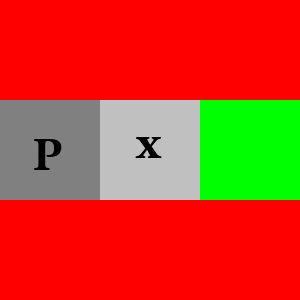
\includegraphics[width=0.5\linewidth]{droit.png}
\caption{Élagage horizontal}
\end{subfigure}
\begin{subfigure}{.3\textwidth}
\centering
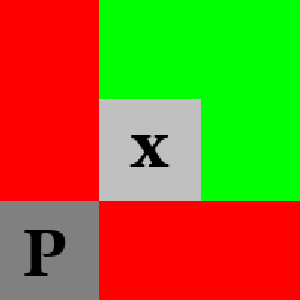
\includegraphics[width=0.5\linewidth]{diag.png}
\caption{Élagage diagonal}
\end{subfigure}
\begin{subfigure}{.3\textwidth}
\centering
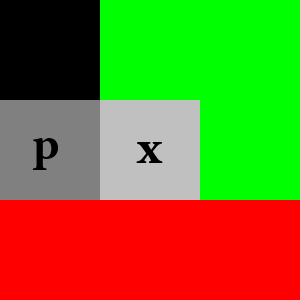
\includegraphics[width=0.5\linewidth]{obstacle.png}
\caption{Cas d'un obstacle}
\end{subfigure}
\caption{En rouge, les voisin éliminés, en vert, les voisin à explorer, en noir, les obstacles, en gris clair, le point courant, en gris foncé le point d'origine}
\end{figure}

Dans le cas où l'exploration dans la direction courante est arrêtée par un obstacle, le chemin y menant depuis le dernier 
changement de direction est purement oublié.

Toutefois, la direction courante est privilégiée, et les voisin induisant un changement de direction ne sont explorés que si
la poursuite de l'exploration de la direction courante échoue.
\end{description}

Enfin, l'algorithme A* est appliqué à chacun des nœuds marqués par JPS jusqu'à trouver le point cible, qui est alors relié au 
nœud qui a permis de le trouver. Enfin, il ne reste plus qu'à remonter le chemin à l'envers pour retrouver le chemin optimal 
du départ à l'arrivée.
\section{Implémentation}
Nous avons décidé d'implémenter le cœur de l'algorithme en C afin de bénéficier au mieux de la rapidité des langages compilés.

Toutefois, dans le but de simplifier son utilisation et son interfaçage avec des programmes de test, nous avons écrit un 
\emph{wrapper} python qui nous permet de profiter de la vitesse de l'algorithme implémenté en C avec la facilité de développement 
et de debuggage d'un langage haut niveau comme python.

C'est ainsi que nous avons pu développer rapidement et simplement les programmes de démonstration inclus dans notre projet.


\end{document}
